\documentclass[12pt, a4paper]{article}
\usepackage{../../../myconfig_line} % Gọi file cấu hình từ ngoài gốc vào
% ==========================================
% BẮT ĐẦU NỘI DUNG TÀI LIỆU
% ==========================================
\begin{document}

% Truyền 3 tham số: {Nhãn cam} {Chữ to chính giữa} {Chữ ở góc phải Header}
\titlebox{Chủ đề: Tích phân}{Ứng dung tích phân tính thể tích hình phẳng thực tế}{Nguyên hàm - Tích phân: Ứng dụng}

\questionTrueFalse{12}{1}{Một kỹ sư A thiết kế một mô hình đường hầm như bên dưới. Biết rằng đường hầm mô hình có chiều dài 5 (m). Khi cắt mô hình này bởi các mặt phẳng vuông góc với đáy của nó, ta được thiết diện là một hình parabol có độ dài đáy gấp đôi chiều cao của parabol (như hình vẽ). Diện tích của thiết diện là \( S(x) \) và chiều cao của mỗi thiết diện parabol cho bởi công thức 
\(h = 3 - \dfrac{2}{5}x\)
với \( x \) (mét) là khoảng cách tính từ lối vào lớn hơn của đường hầm mô hình đến mặt phẳng chứa thiết diện.

\begin{figure}[H]
    \centering
    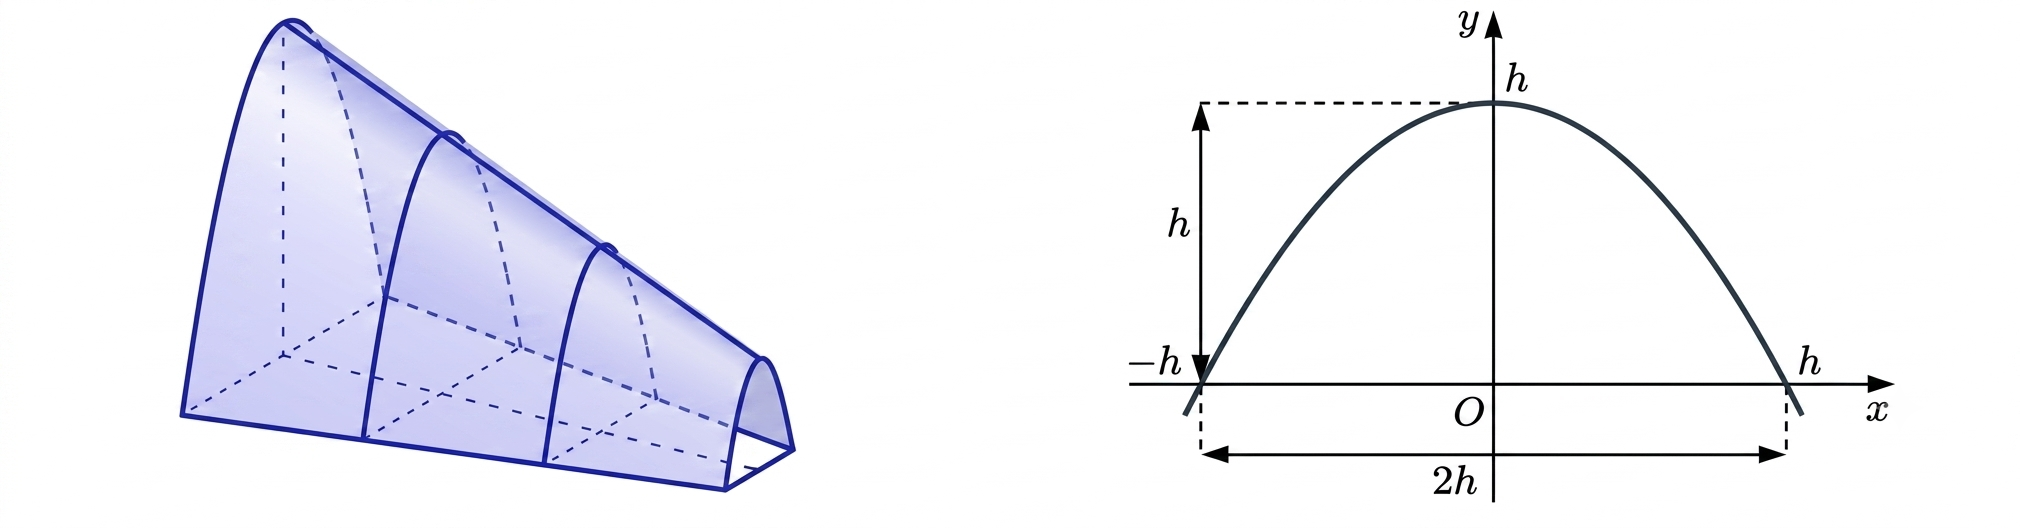
\includegraphics[width=0.9\textwidth]{../images/Ham.png}
\end{figure}
}{
    \textbf{a)} & Diện tích thiết diện được tính bởi công thức 
    \(S = 2 \displaystyle\int_{0}^{h} \left( h - \dfrac{x^2}{h} \right) dx.\)
    & \textcolor{amberorange}{$\bigcirc$} & \textcolor{amberorange}{$\bigcirc$} \\ \hline
    
    \textbf{b)} & Thể tích của đường hầm được tính theo công thức: 
    \(V = \pi \displaystyle\int_{0}^{5} S^2(x) dx \quad (m^3).\)
    & \textcolor{amberorange}{$\bigcirc$} & \textcolor{amberorange}{$\bigcirc$} \\ \hline
    
    \textbf{c)} & Parabol có chiều cao \( h \), độ dài đáy bằng \( 2h \) có phương trình là 
    \(y = -\dfrac{x^2}{h} + h.\)
    & \textcolor{amberorange}{$\bigcirc$} & \textcolor{amberorange}{$\bigcirc$} \\ \hline
    
    \textbf{d)} & Thể tích của hầm là \( 29,89 \left( m^3 \right) \) (làm tròn đến hàng phần trăm).
    & \textcolor{amberorange}{$\bigcirc$} & \textcolor{amberorange}{$\bigcirc$} \\
}

\questionShortAnswer{20}{2}{Để đặt được một vật trang trí trên mặt bàn, người ta thiết kế một chân đế như sau. Lấy một khối gỗ có dạng khối chóp cụt tứ giác đều với độ dài hai cạnh đáy lần lượt bằng \( 7,4 \, \text{cm} \) và \( 10,4 \, \text{cm} \), bề dày khối gỗ bằng \( 1,5 \, \text{cm} \). Sau đó khoét bỏ đi một phần của khối gỗ sao cho phần đó có dạng vật thể \( H \), ở đó \( H \) nhận được bằng cách cắt khối cầu bán kính \( 5,5 \, \text{cm} \) bởi một mặt phẳng cắt mà mặt cắt là hình tròn bán kính \( 3,5 \, \text{cm} \) (xem hình dưới). 

\begin{center}
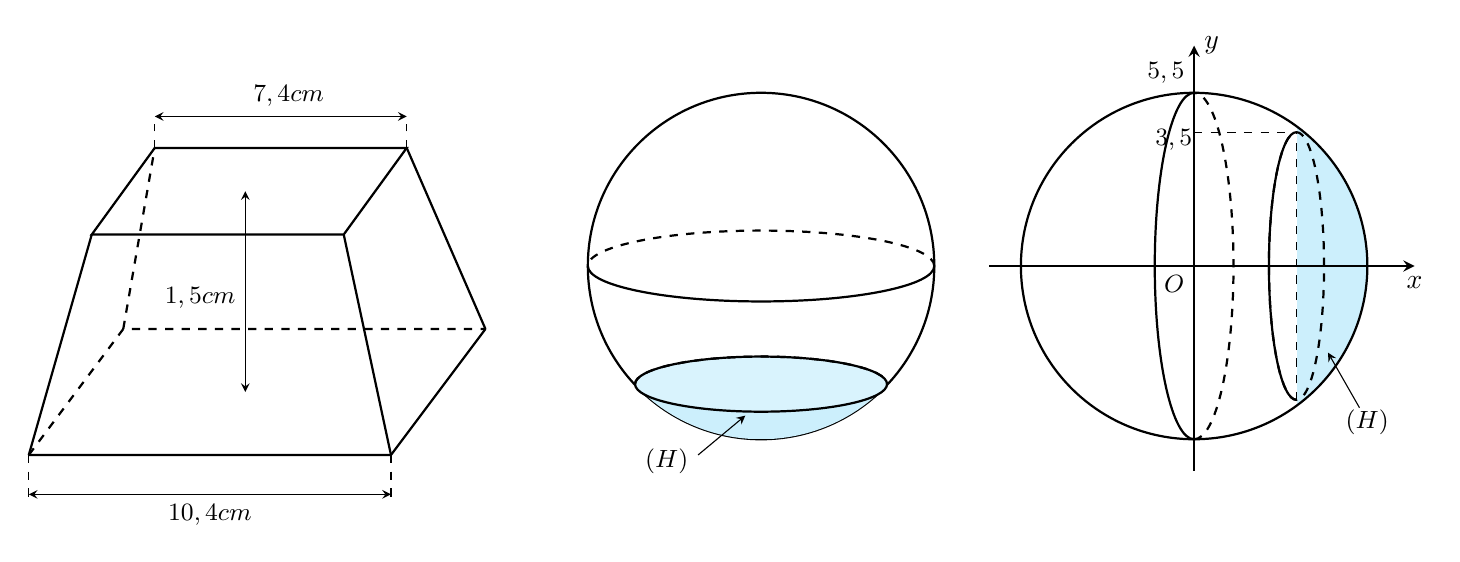
\begin{tikzpicture}[scale=1, >=latex]

    % ==========================================
    % HÌNH 1: KHỐI CHÓP CỤT TÚ GIÁC ĐỀU (BÊN TRÁI)
    % ==========================================
    \begin{scope}[shift={(-6.5, 0)}]
        % Tọa độ đáy lớn (độ dài 10,4 cm)
        \coordinate (A) at (-2.8, -1.2);
        \coordinate (B) at (1.8, -1.2);
        \coordinate (C) at (3.0, 0.4);
        \coordinate (D) at (-1.6, 0.4);

        % Tọa độ đáy nhỏ (độ dài 7,4 cm)
        \coordinate (A1) at (-2.0, 1.6);
        \coordinate (B1) at (1.2, 1.6);
        \coordinate (C1) at (2.0, 2.7);
        \coordinate (D1) at (-1.2, 2.7);

        % Các cạnh khuất (nét đứt)
        \draw[thick, dashed, black] (A) -- (D) -- (C);
        \draw[thick, dashed, black] (D) -- (D1);

        % Các cạnh nhìn thấy (nét liền)
        \draw[thick, black] (A) -- (B) -- (C);
        \draw[thick, black] (A1) -- (B1) -- (C1) -- (D1) -- cycle;
        \draw[thick, black] (A) -- (A1);
        \draw[thick, black] (B) -- (B1);
        \draw[thick, black] (C) -- (C1);

        % Chiều cao 1,5 cm
        \coordinate (O_top) at (0, 2.15);
        \coordinate (O_bot) at (0, -0.4);
        
        \draw[<->, >=stealth, black] (-0.05, -0.4) -- (-0.05, 2.15);
        \node[left, font=\small] at (-0.05, 0.8) {$1,5\text{cm}$};

        % Đường kích thước đáy trên (7,4 cm)
        \draw[dashed, black] (D1) -- (-1.2, 3.0);
        \draw[dashed, black] (C1) -- (2, 3.0);
        \draw[<->, >=stealth, black] (-1.2, 3.1) -- (2, 3.1);
        \node[above, font=\small] at (0.5, 3.1) {$7,4\text{cm}$};

        % Đường kích thước đáy dưới (10,4 cm)
        \draw[dashed, black] (A) -- (-2.8, -1.8);
        \draw[dashed, black] (B) -- (1.8, -1.8);
        \draw[<->, >=stealth, black] (-2.8, -1.7) -- (1.8, -1.7);
        \node[below, font=\small] at (-0.5, -1.7) {$10,4\text{cm}$};
    \end{scope}

    % ==========================================
    % HÌNH 2: KHỐI CẦU VÀ CHỎM CẦU (Ở GIỮA)
    % ==========================================
    \begin{scope}[shift={(0, 1.2)}]
        \pgfmathsetmacro{\R}{2.2} % Bán kính cầu trên hình

        % Đường tròn lớn của khối cầu
        \draw[thick, black] (0,0) circle (\R);

        % Vĩ tuyến xích đạo (nét đứt sau, nét liền trước)
        \draw[thick, dashed, black] (\R, 0) arc (0:180:\R cm and 0.45cm);
        \draw[thick, black] (-\R, 0) arc (180:360:\R cm and 0.45cm);

        % Chỏm cầu (H) ở dưới đáy
        \begin{scope}
            \clip (0,0) circle (\R);
            \fill[cyan!20] (-\R, -1.5) rectangle (\R, -\R);
        \end{scope}

        % Đường cắt của chỏm cầu (elip)
        \draw[thick, black, fill=cyan!15] (0, -1.5) ellipse (1.6cm and 0.35cm);
        \draw[thick, dashed, black] (-1.6, -1.5) arc (180:0:1.6cm and 0.35cm);

        % Nhãn (H)
        \draw[->, >=stealth, black] (-0.8, -2.4) -- (-0.2, -1.9);
        \node[below left, font=\small\itshape] at (-0.8, -2.2) {$(H)$};
    \end{scope}

    % ==========================================
    % HÌNH 3: HỆ TRỤC TỌA ĐỘ Oxy (BÊN PHẢI)
    % ==========================================
    \begin{scope}[shift={(5.5, 1.2)}]
        \pgfmathsetmacro{\R}{2.2}

        % Tô màu chỏm cầu (H) bên phải
        \begin{scope}
            \clip (0,0) circle (\R);
            \fill[cyan!20] (1.3, -\R) rectangle (\R, \R);
        \end{scope}

        % Hệ trục tọa độ Oxy
        \draw[->, >=stealth, thick, black] (-2.6, 0) -- (2.8, 0) node[below] {$x$};
        \draw[->, >=stealth, thick, black] (0, -2.6) -- (0, 2.8) node[right] {$y$};
        \node[below left, font=\small] at (0, 0) {\small$O$};

        % Đường tròn R = 5.5
        \draw[thick, black] (0,0) circle (\R);

        % Kinh tuyến đứng (nét đứt sau, nét liền trước)
        \draw[thick,  black] (0, \R) arc (90:270:0.5cm and \R cm);
        \draw[thick,dashed, black] (0, -\R) arc (-90:90:0.5cm and \R cm);

        % Mặt cắt hình tròn bán kính 3.5 (ở x = x_cut)
        \draw[thick,dashed, black] (1.3, 0) ellipse (0.35cm and 1.7cm);
        \draw[thick, black] (1.3, 1.7) arc (90:270:0.35cm and 1.7cm);

        % Nhãn giá trị trên trục y (5,5 và 3,5)
        \node[above left, font=\small] at (0, \R) {$5,5$};
        \draw[dashed, black] (0, 1.7) -- (1.3, 1.7);
        \node[left, font=\small] at (0.1, 1.6) {$3,5$};
        \draw[dashed, black] (1.3, -1.7) -- (1.3, 1.7);

        % Nhãn (H)
        \draw[->, >=stealth, black] (2.1, -1.8) -- (1.7, -1.1);
        \node[below right, font=\small\itshape] at (1.8, -1.7) {$(H)$};
    \end{scope}

\end{tikzpicture}
\end{center}


Thể tích của khối chân đế bằng bao nhiêu centimét khối (không làm tròn kết quả các phép tính trung gian, chỉ làm tròn kết quả cuối cùng đến hàng phần mười).

}




\questionShortAnswer{23}{3}{Một lều cắm trại có dạng như hình vẽ dưới, khung lều được tạo thành từ hai parabol giống nhau có chung đỉnh \( O \) và thuộc hai mặt phẳng vuông góc nhau (một parabol đi qua \( A, O, C \) và một parabol đi qua \( B, D, O \)), bốn chân tạo thành hình vuông \( ABCD \) có cạnh là \( 2\sqrt{2} \) (m), chiều cao tính từ đỉnh lều là \( 2 \) (m). Biết mặt cắt của lều khi cắt bởi một mặt phẳng song song với mặt phẳng \( (ABCD) \) luôn là một hình vuông. Tính thể tích của lều (đơn vị là \( m^3 \)).

\begin{figure}[H]
    \centering
    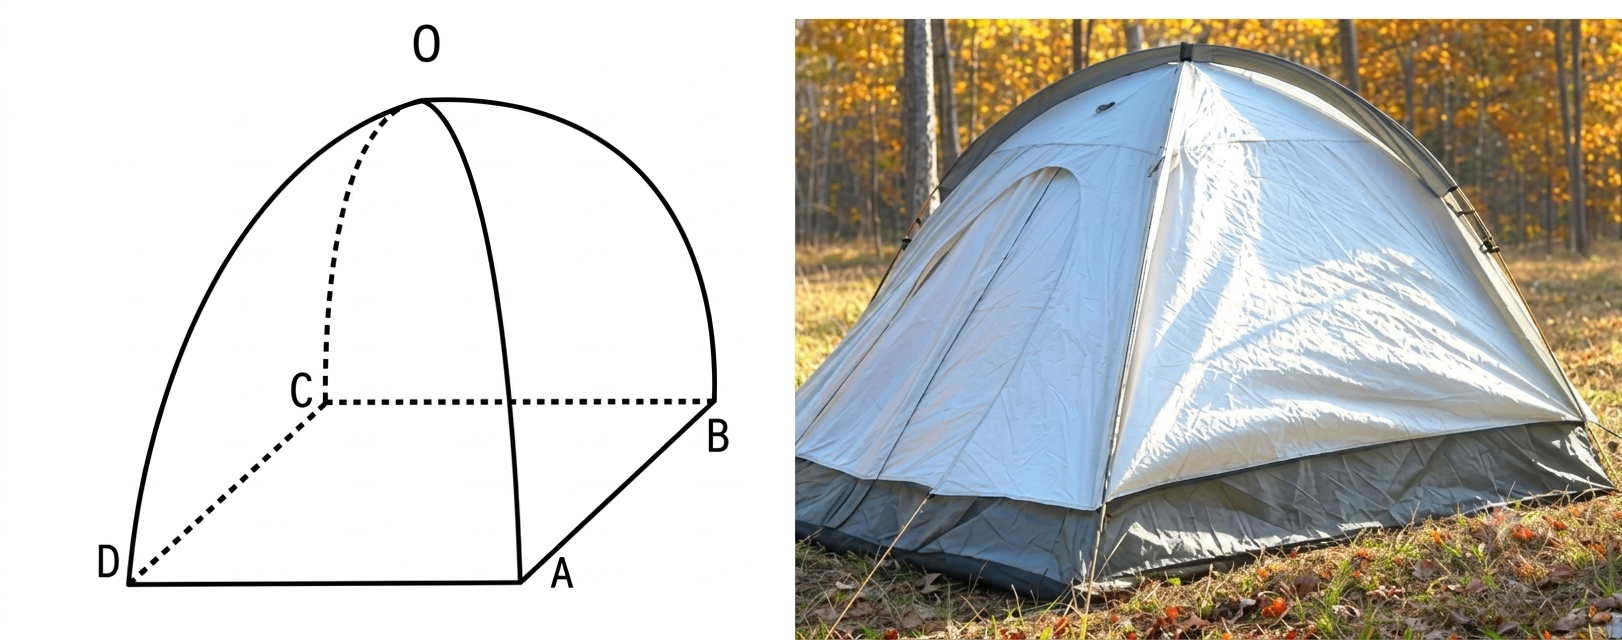
\includegraphics[width=0.8\textwidth]{../images/Leu.png}
\end{figure}

}

\questionShortAnswer{20}{4}{Một ly trà sữa dạng hình nón cụt, có đường kính đáy ly 6cm, đường kính miệng ly 9cm, chiều cao 13,4cm, ở miệng ly có sử dụng một nắp đậy có hình dạng nửa mặt cầu và ở đỉnh của nửa mặt cầu này có một hình tròn có đường kính 2cm để cắm ống hút, mặt phẳng chứa hình tròn này song song với mặt phẳng chứa miệng ly (tham khảo hình vẽ sau).  
\begin{figure}[H]
    \centering
    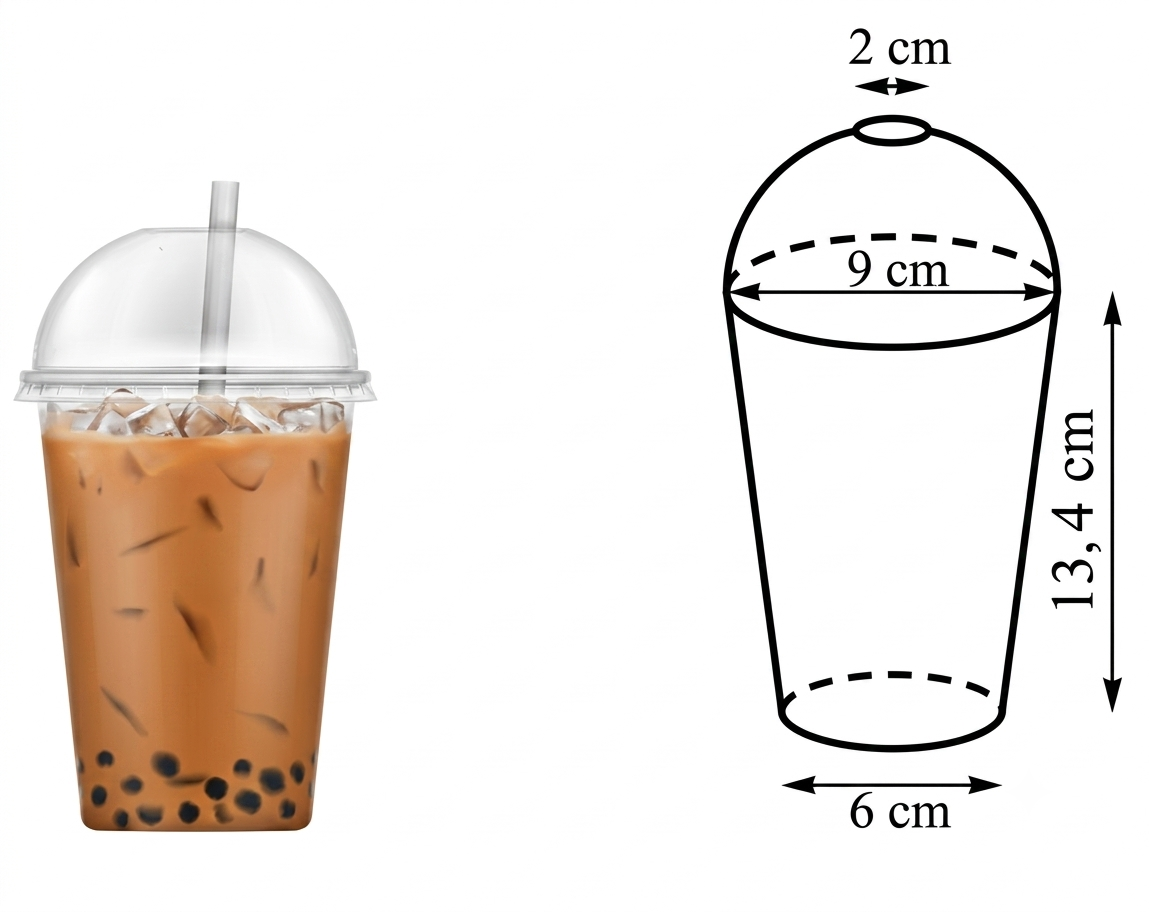
\includegraphics[width=0.4\textwidth]{../images/TraSua.png}
\end{figure}

Thể tích bên trong của ly bao gồm cả thể tích của nắp là bao nhiêu cm\(^3\)? (làm tròn kết quả đến hàng đơn vị).

}




\questionShortAnswer{20}{5}{Một kiến trúc sư chịu trách nhiệm thiết kế một tòa nhà cao 30 mét. Mặt cắt ngang tại mọi độ cao, vuông góc với trục thẳng đứng, luôn là một hình vuông (xem hình vẽ).

\begin{figure}[H]
    \centering
    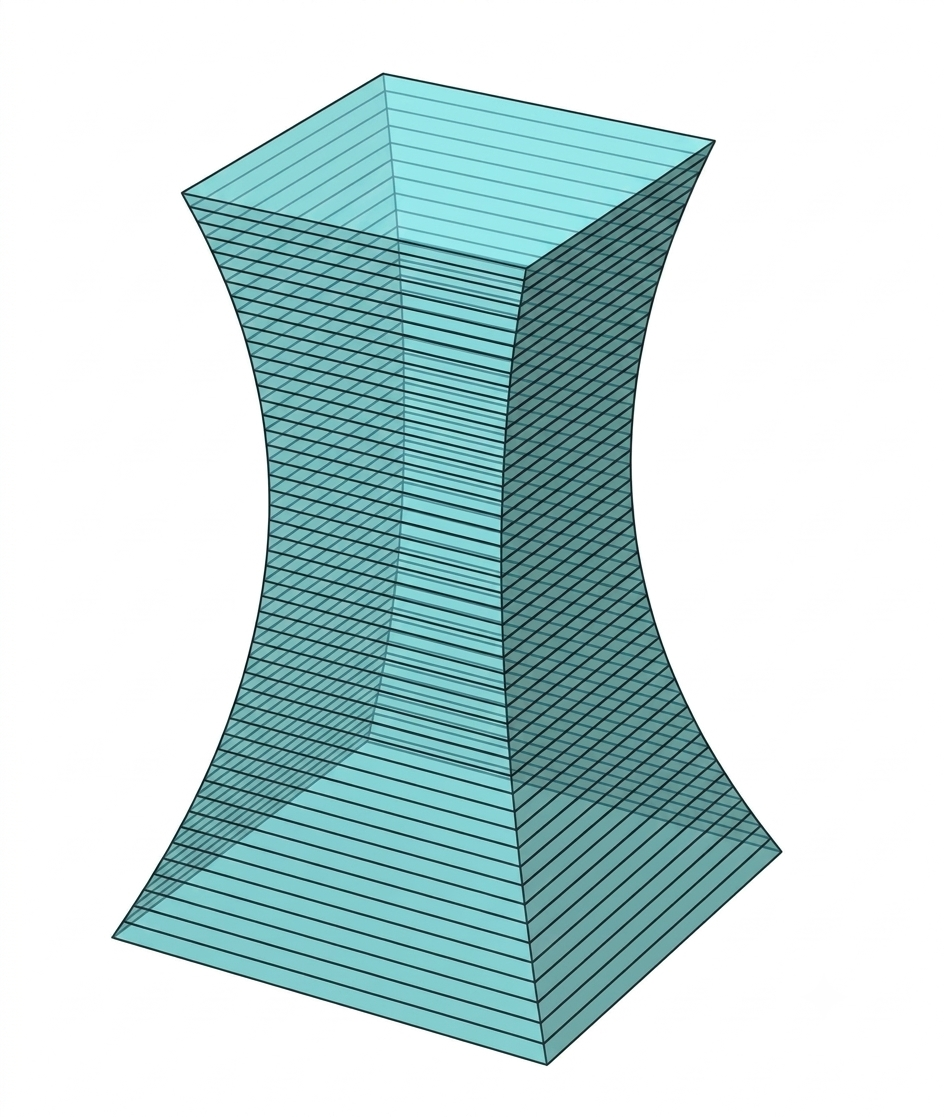
\includegraphics[width=0.3\textwidth]{../images/ToaNha.png}
\end{figure}

Mặt đáy tòa nhà là hình vuông có cạnh \( L_0 = 26 \, \text{m} \), mặt đỉnh là hình vuông có cạnh \( L_{30} = 20 \, \text{m} \).  
Mặt cắt ngang tại vị trí hẹp nhất của tòa nhà: Hình vuông có cạnh \( L_{min} = 13,75 \, \text{m} \). Mặt cắt của tòa nhà theo mặt phẳng đứng chứa đường chéo đáy có dạng là hình phẳng giới hạn bởi hai đường cong parabol đối xứng nhau qua trục thẳng đứng đi qua tâm đáy của tòa nhà. Tính thể tích của tòa nhà đó (làm tròn đến hàng đơn vị, đơn vị tính: mét khối).

}

\questionShortAnswer{23}{6}{Một bồn hình trụ đang chứa dầu, được đặt nằm ngang, có chiều dài bồn là 5m, có bán kính đáy 1m. Người ta đã rút dầu trong bồn tương ứng với 0,5m của đường kính đáy. Tính thể tích của lượng dầu còn lại trong bồn theo đơn vị \( m^3 \). (làm tròn đến hàng phần chục)
\begin{center}
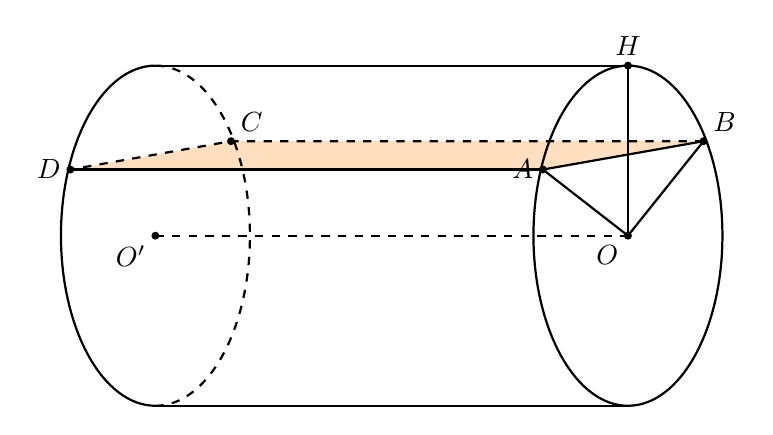
\begin{tikzpicture}[scale=1.2, >=latex]

    % 1. Định nghĩa các tọa độ chuẩn:
    % Tâm O (đáy phải), O' (đáy trái)
    \coordinate (O)  at (3, 0);
    \coordinate (O1) at (-2, 0); % O'

    % Mặt cắt dầu ABCD
    \coordinate (A) at (2.1, 0.7);
    \coordinate (B) at (3.8, 1);
    \coordinate (C) at (-1.2, 1);
    \coordinate (D) at (-2.9, 0.7);

    % Đỉnh cao nhất của đường kính H
    \coordinate (H) at (3, 1.8);

    % 2. Tô màu mặt cắt dầu ABCD
    \fill[orange!25] (A) -- (B) -- (C) -- (D) -- cycle;

    % 3. Vẽ thành bồn hình trụ nằm ngang
    % Đường sinh trên và dưới
    \draw[thick, black] (-2, 1.8) -- (3, 1.8);
    \draw[thick, black] (-2, -1.8) -- (3, -1.8);

    % Đáy phải (nét liền)
    \draw[thick, black] (O) ellipse (1cm and 1.8cm);

    % Đáy trái (nửa trước nét liền, nửa sau nét đứt)
    \draw[thick, dashed, black] (-2, -1.8) arc (-90:90:1cm and 1.8cm);
    \draw[thick, black] (-2, 1.8) arc (90:270:1cm and 1.8cm);

    % 4. Vẽ các đường nét đứt và nét liền chi tiết
    % Trục nối hai tâm O - O'
    \draw[thick, dashed, black] (O1) -- (O);

    % Hình chữ nhật ABCD (mặt cắt dầu)
    \draw[thick, black] (A) -- (B);
    \draw[thick, black] (A) -- (D);
    \draw[thick, dashed, black] (B) -- (C) -- (D);

    % Đường kính dọc OH và các bán kính OA, OB
    \draw[thick, black] (O) -- (H);
    \draw[thick, black] (O) -- (A);
    \draw[thick, black] (O) -- (B);

    % 5. Đánh dấu điểm và nhãn
    \fill[black] (O)  circle (1.2pt) node[below left] {$O$};
    \fill[black] (O1) circle (1.2pt) node[below left] {$O'$};
    \fill[black] (H)  circle (1.2pt) node[above] {$H$};
    \fill[black] (A)  circle (1.2pt) node[left] {$A$};
    \fill[black] (B)  circle (1.2pt) node[above right] {$B$};
    \fill[black] (C)  circle (1.2pt) node[above right] {$C$};
    \fill[black] (D)  circle (1.2pt) node[left] {$D$};

\end{tikzpicture}
\end{center}
}


\end {document}
